% ============================================================================
% WP2: Floquet-guided causal stabilization (article-Max insertion)
% Requires the figures and tables shipped with the WP2 archive.
% ============================================================================
\section{Floquet-guided causal stabilization}
\label{sec:control}

The spectral calculations identify an unstable edge subspace, but correlation
alone does not establish that this subspace causes the forward Nyquist packets.
We therefore introduce two interventions. The first is an orbit-preserving
fourth-difference damping used to continue the edge--Floquet spectrum through
the unit circle. The second is ordinary total-state hyperviscosity, used to test
whether the corresponding threshold suppresses the packets without materially
changing the resolved compacton.

Let
\begin{equation}
 D_4=E^{-2}-4E^{-1}+6-4E+E^2.
\end{equation}
Because ordinary hyperviscosity dissipates the compacton slowly, the dissipative
scheme has no nonzero exactly periodic traveling orbit of fixed amplitude. To
define an unambiguous spectral continuation, at midpoint substep $k$ we use
\begin{equation}
 \cA\frac{U^{k+1}-U^k}{\Delta t}
 +(\cB+\cC)\Phi(\bar U^k)
 +\varepsilon D_4(\bar U^k-\bar U_*^k)=0,
 \label{eq:orbitpreservinghyper}
\end{equation}
where $\bar U_*^k$ is the corresponding midpoint on the undamped traveling
orbit. Equation~\eqref{eq:orbitpreservinghyper} leaves $U_*$ fixed exactly and
has the same linear fourth-difference damping of perturbations as the ordinary
hyperviscous scheme. Its tangent substep is
\begin{equation}
 T_k^{(\varepsilon)}=
 \left[\frac{\cA}{\Delta t}+(\cB+\cC)D_k+\frac{\varepsilon}{2}D_4\right]^{-1}
 \left[\frac{\cA}{\Delta t}-(\cB+\cC)D_k-\frac{\varepsilon}{2}D_4\right].
 \label{eq:controlledtangent}
\end{equation}

Continuation of the edge-localized spectrum gives
\begin{equation}
 \varepsilon_c=0.36875\pm0.00125
 \quad(h=0.01,\ \kappa=5),
 \qquad
 \varepsilon_c=0.19097\pm0.00125
 \quad(h=0.02,\ \kappa=20).
 \label{eq:epscritical}
\end{equation}
The first crossing is through the real negative branch. In the second case the
real mode is stabilized first and a complex-conjugate edge pair determines the
final crossing. In terms of the Nyquist damping accumulated in one cell
crossing, $\delta_N=120\varepsilon h$, the two thresholds are $0.4425$ and
$0.4583$, respectively.

\begin{figure}[t]
 \centering
 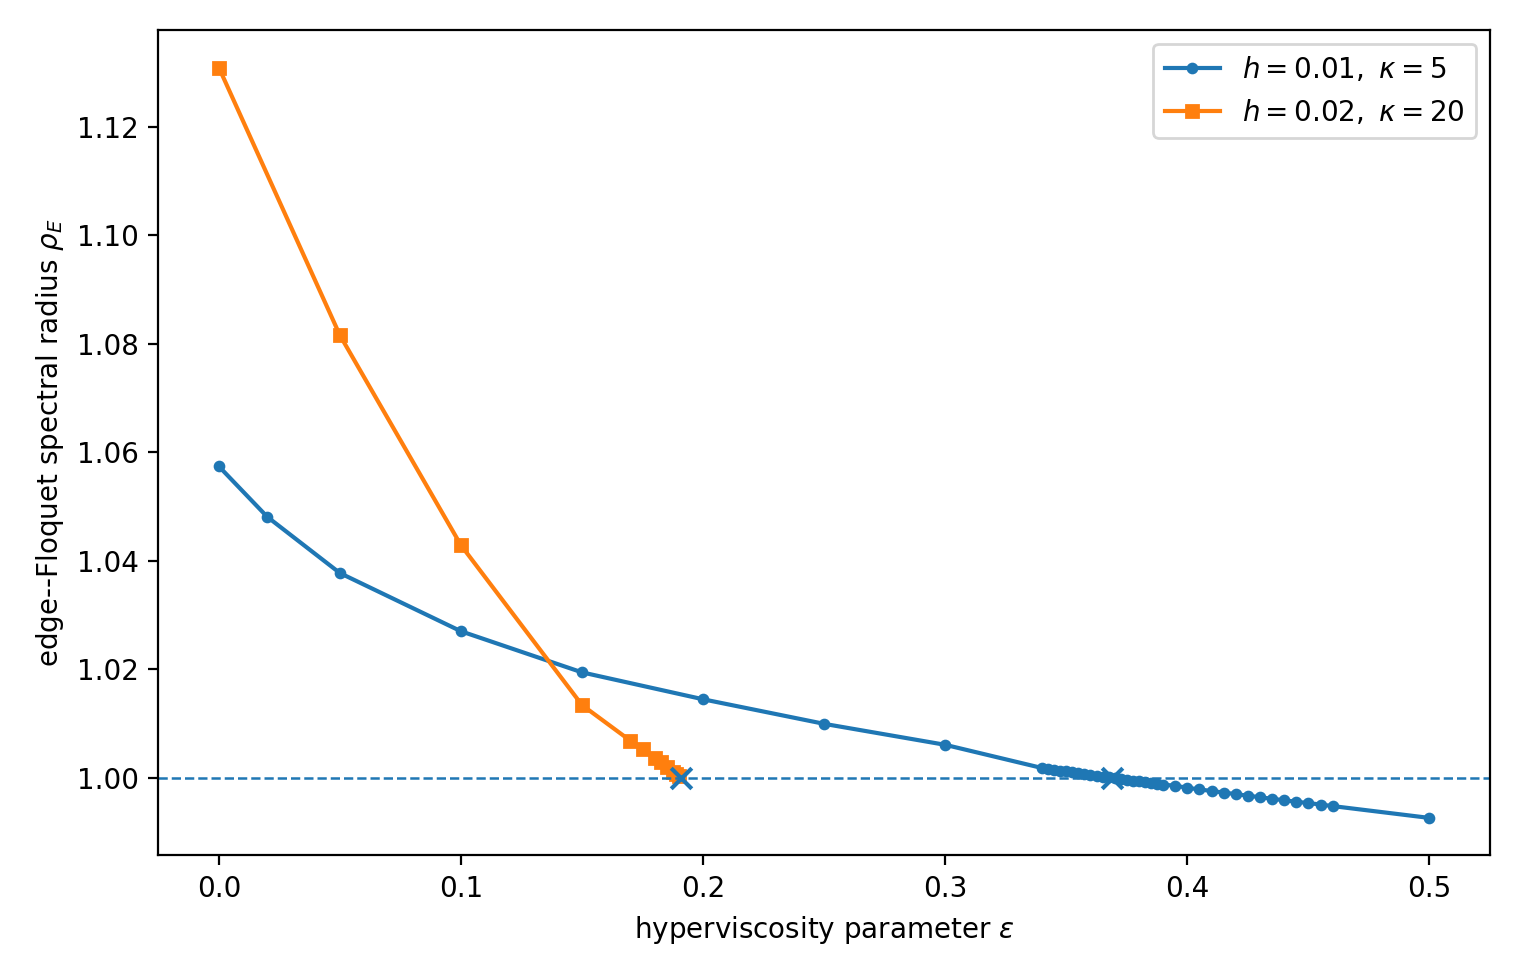
\includegraphics[width=.72\textwidth]{wp2_hyperviscosity_floquet_continuation.png}
 \caption{Orbit-preserving hyperviscous continuation of the dominant
 edge--Floquet spectral radius. The horizontal line is the neutral boundary.
 For $h=0.02$, $\kappa=20$, a complex pair controls the final crossing.}
 \label{fig:hypercontinuation}
\end{figure}

The same parameter values were then inserted into the ordinary total-state
scheme. At $\varepsilon\simeq\varepsilon_c$, the maximum forward high-pass
amplitude is reduced by factors of approximately $8.0\times10^2$ and
$1.3\times10^3$ in the two principal cases. By contrast,
$\varepsilon=10^{-5}$ does not suppress the instability. The mass is conserved
to roundoff; the maximum relative changes of the compacton peak and quadratic
norm remain below $10^{-8}$ over the reported intervals. Hence the suppression
is not caused by an appreciable damping or deformation of the resolved
compacton core.

\begin{figure}[t]
 \centering
 \begin{minipage}{.49\textwidth}\centering
  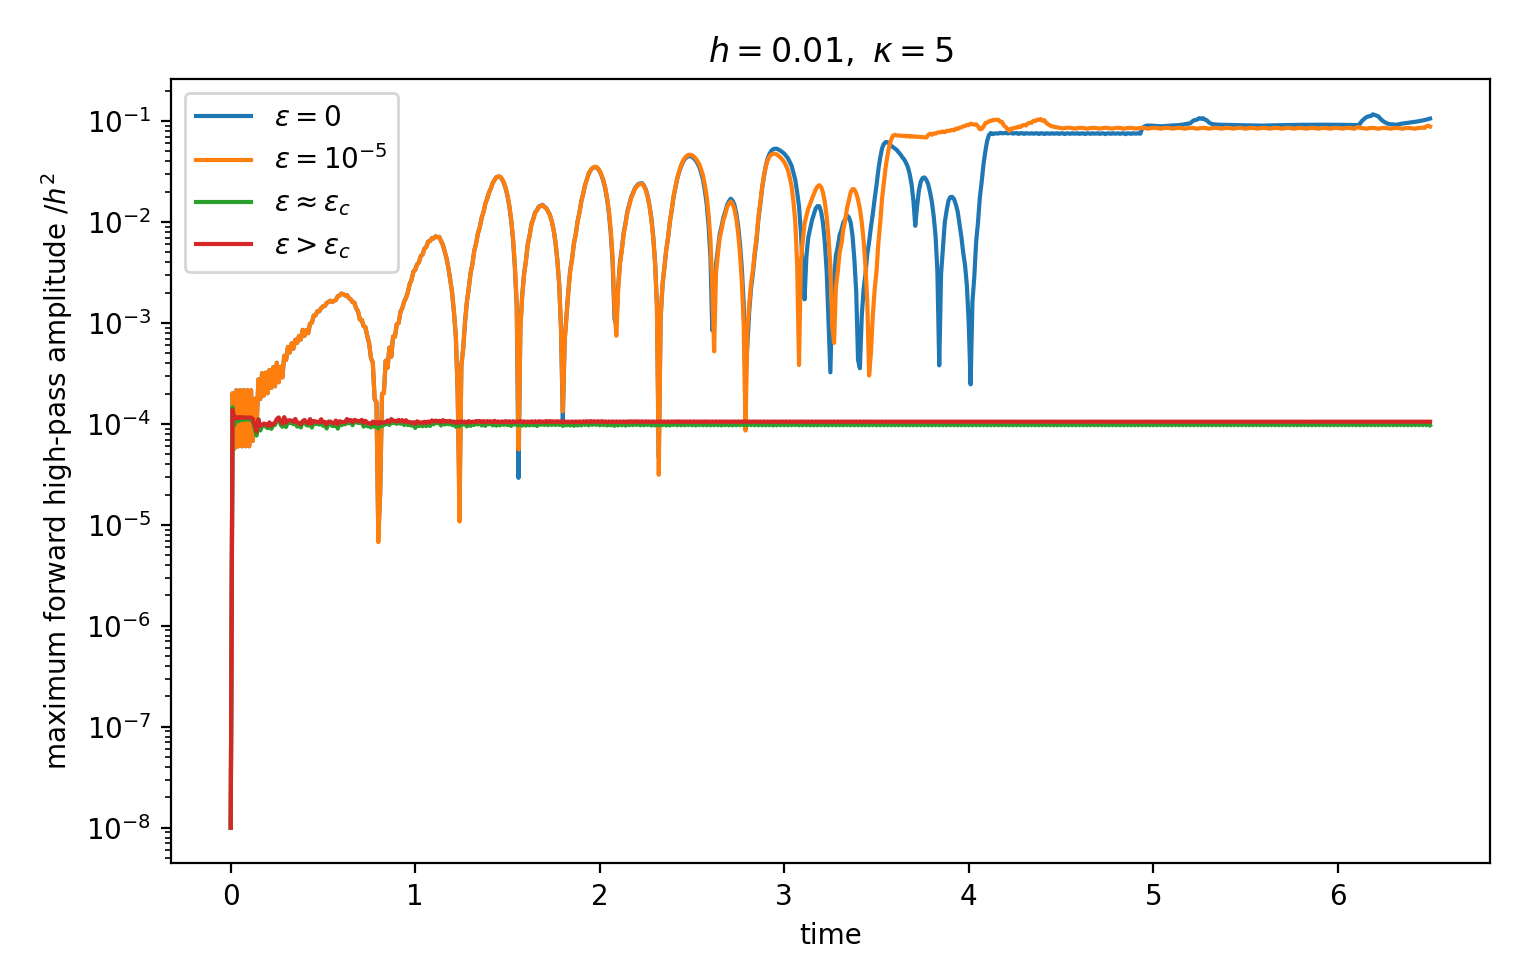
\includegraphics[width=\linewidth]{wp2_ordinary_hyperviscosity_suppression_h001_k5.png}
 \end{minipage}\hfill
 \begin{minipage}{.49\textwidth}\centering
  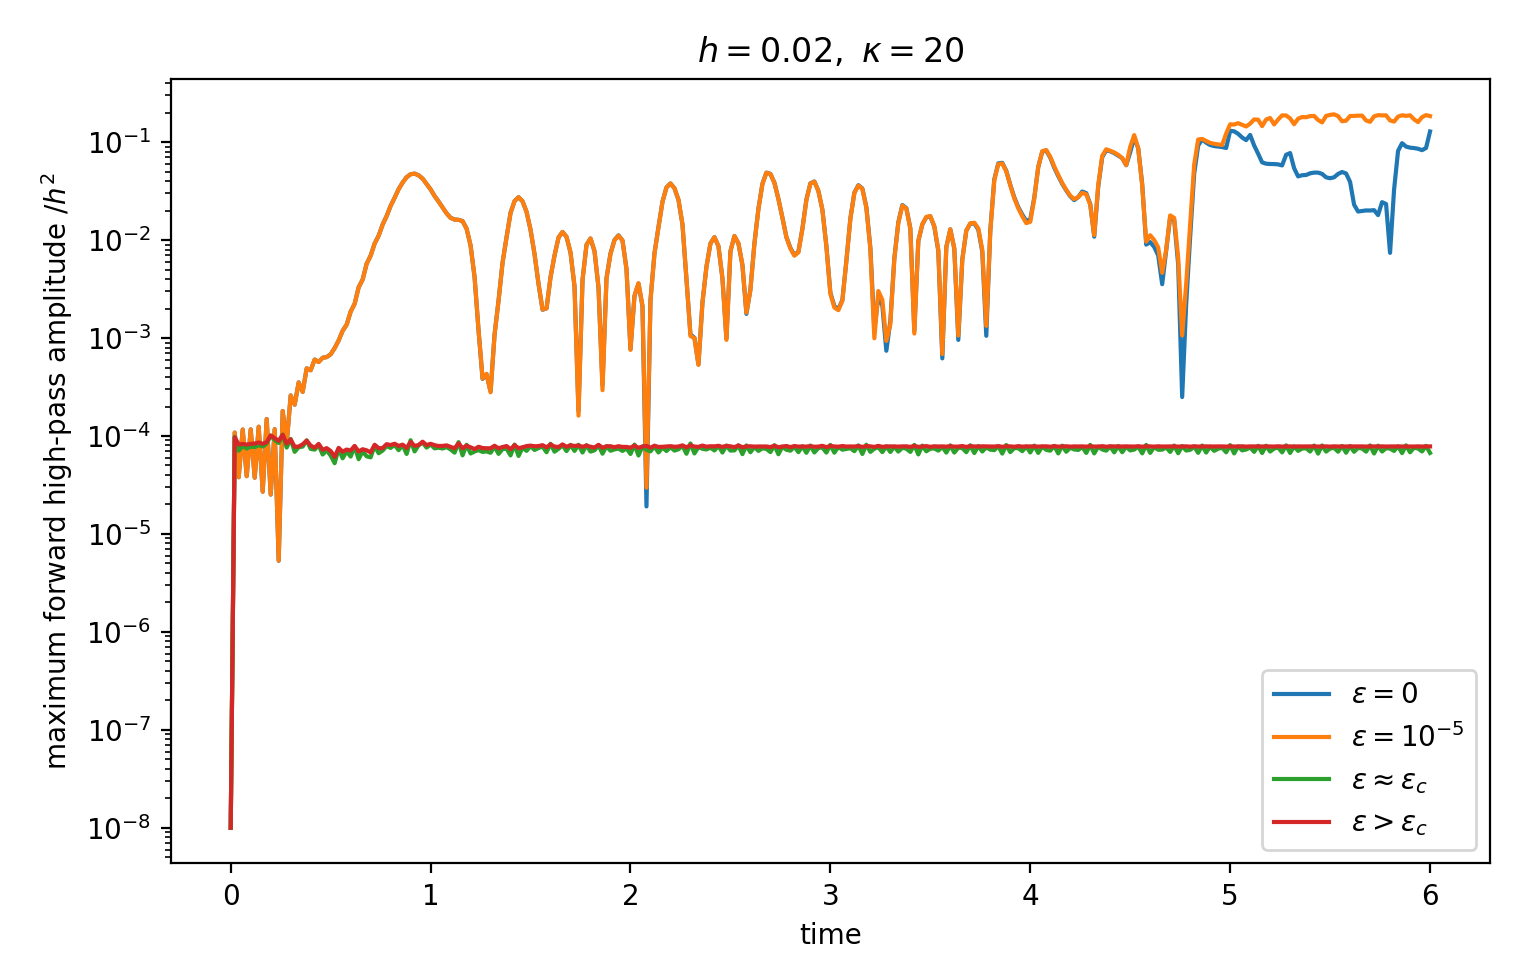
\includegraphics[width=\linewidth]{wp2_ordinary_hyperviscosity_suppression_h002_k20.png}
 \end{minipage}
 \caption{Forward high-frequency amplitude under ordinary total-state
 hyperviscosity. Damping at the Floquet-predicted threshold suppresses the
 emitted Nyquist packets by about three orders of magnitude, whereas the small
 value used in earlier compacton calculations does not.}
 \label{fig:hypersuppression}
\end{figure}

As a sharper diagnostic, let $R$ and $L$ span the unstable right and left
Floquet subspaces, and set
\begin{equation}
 \Pi_u=R(L^TR)^{-1}L^T.
\end{equation}
The controlled one-cell map
\begin{equation}
 \cP_\alpha(U)=U_*+[I-\alpha\Pi_u]
 [\cP_{\rm NL}(U)-U_*]
 \label{eq:modalcontrol}
\end{equation}
multiplies every selected unstable multiplier by $1-\alpha$. For
$h=0.02$, $\kappa=20$, damping only the leading real mode is insufficient,
because a complex unstable pair remains. Damping the complete three-dimensional
real unstable subspace reduces the forward packet amplitude by a factor of
about $59$; full projection removal drives the unstable coordinates to
roundoff. This establishes that the complete unstable edge subspace, rather
than a single scalar mode, is the relevant causal object.

A one-time removal of the leading component from the initial condition does not
prevent later shedding: nonnormal coupling and the remaining edge spectrum
repopulate it. Continuous stabilization is therefore required. Together, the
spectral crossing, eigenmode-seeded growth/decay, ordinary-hyperviscosity test,
and unstable-subspace control provide independent causal evidence for the
Floquet mechanism.
